\subsection{Computational requirements} \label{sec:vcgenres}
While the key computational concern of motion planning using primitives is the on-line cost, the computational requirements of the off-line library generation are still relevant; the library must be generated in some reasonable interval or else it forms a bottleneck in the development time of a dynamic walking robot.

Recall from Section \ref{sec:lib} that the size of the virtual constraint library is $n_k(n_xn_yn_q)^2$. Therefore, even in the simple case of the compass-gait robot, a library which provides sufficiently fine coverage of motions to suit general terrains requires a very large number of virtual constraints. To illustrate this, a library was generated for the compass-gait robot which has $n_x=5,n_y=11$ and $n_k=11$, resulting in 33 275 virtual constraints. Fortunately, the outer loop of Algorithm \ref{alg:highlevellib} is able to be computed in parallel. On a modern quad-core desktop computer running MATLAB, this library was completed in 46 830 s ($\approx$ 13 h). The storage requirement for the library was 6.85 MB, which is insignificant in comparison to the computational time. Note that since the algorithm is parallel and there are platforms which are much more efficient than MATLAB, the construction of a large number of primitives is not prohibitively challenging.

\subsection{Velocity ordering of VCs in optimised library}
As discussed in Section \ref{sec:orderings}, if the library contains primitives which have $\Gamma(\theta^c)$ and $\Psi(\theta^c)$ structured similarly to Figure \ref{fig:totord}, the ordering method introduced in Section \ref{sec:orderings} becomes independent of the target velocity. This is favourable, since the heuristics set a target velocity (or energy), therefore other than for the unguided best-first search, a target velocity-specific ordering is of limited utility.

The feasibility of ordering the set of constraints, it would seem, is quite dependent on the particular set within the library. For example, constraints which are suitable for walking on flat ground, i.e. $s_h=0$, typically have a similar structure to that shown in Figure \ref{fig:GPFlat}. While this contains some points which very poorly match the velocity-independent ordering, relatively few points can be removed to produce a set which does match, since the general trend of the data is a line which has a gradient $<1$.

\begin{figure}
\centering
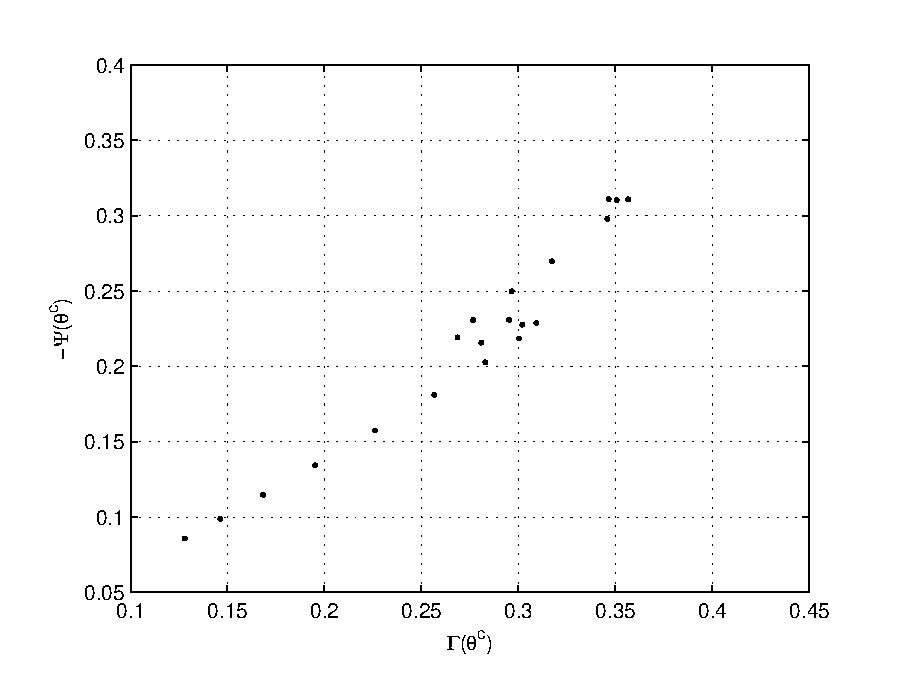
\includegraphics[width=0.6\linewidth]{7Results/GPFlat}
\caption{Typical plot of $\Gamma(\theta^c)$ and $-\Psi(\theta^c)$ for flat ground VCs}
\label{fig:GPFlat}
\end{figure}

For virtual constraints which include a step up or down, the points do not often fall onto the somewhat neat line of the flat ground result. Some sets produce points like in Figure \ref{fig:GPSU}, which is conducive to the velocity independent ordering without any alteration, with the exception of a single point. However others show a systematic shape which violates the condition, as in Figure \ref{fig:GPSD}.

\begin{figure}
\begin{minipage}{0.48\textwidth}
\centering
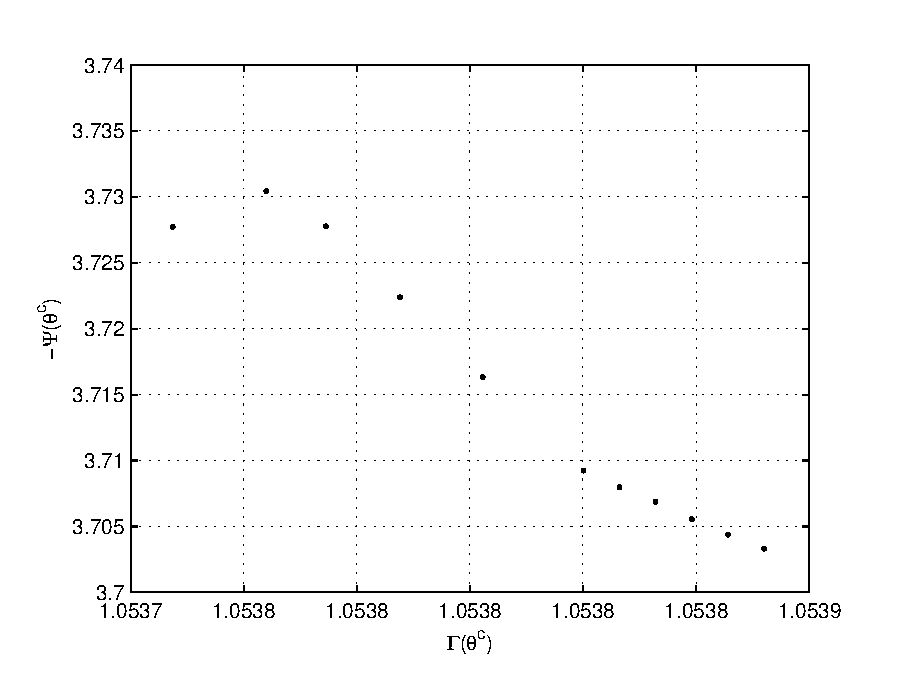
\includegraphics[width=\linewidth]{7Results/GPSU}
\caption{$\Gamma(\theta^c)$ and $-\Psi(\theta^c)$ for a sample step-up trajectory showing good ordering}
\label{fig:GPSU}
\end{minipage}
\hfill
\begin{minipage}{0.48\textwidth}
\centering
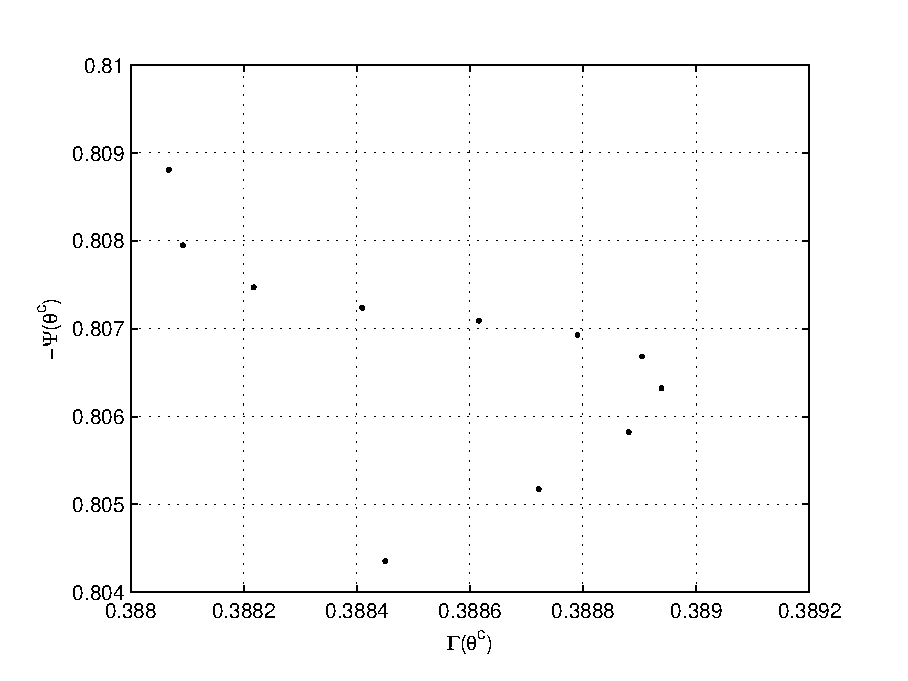
\includegraphics[width=\linewidth]{7Results/GPSD}
\caption{$\Gamma(\theta^c)$ and $-\Psi(\theta^c)$ for a step-down trajectory}
\label{fig:GPSD}
\end{minipage}
\end{figure}

While there does not seem to be any guarantee of structure among the virtual constraints which can be known \textit{a priori}, these results suggest that for the majority of cases, an ordering can be produced which includes most of the virtual constraints. There are numerous methods by which several ordered sets could be extracted from the set of applicable virtual constraints. However, the implementation of such a method and its proof of efficacy are deferred to a later work.

\subsection{Failures}
While the optimisation of the virtual constraints has attempted to be framed in such a way as to ensure feasibility of the optimisation, e.g. by regularisation, the nature of nonlinear optimisation, particularly constrained, means there is no means of ensuring that this is the case for all initial and final conditions.

Failures are undesirable for two reasons. Firstly, they degrade the coverage in the virtual constraint library, since the virtual constraint intended to link the particular initial and final configurations with the desired change in kinetic energy will not exist in the produced library. Secondly, infeasible optimisations typically take a much longer period to terminate than successful well-formed optimisations.

It is not easy to rigorously analyse the rate of failure of the virtual constraint library generation. We are able to produce some result by simply attempting to generate a library and counting the number of failures, as well as observing where those failures tend to occur. Note that we also consider an optimisation to have failed if there is no critical point $\theta^c$ in the interval defined by the virtual constraint.

For the compass-gait library generated as discussed in Section \ref{sec:vcgenres} with 33 275 virtual constraints, 4026 failures were counted, producing a useful library of 29 249 virtual constraints, or an 87.9\% yield. The failures were almost universally produced in virtual constraints which attempted to add kinetic energy whilst also stepping up the terrain. This is not an unexpected result intuitively, particularly for the compass-gait robot.